\documentclass{grand-jeu}
\usepackage{wrapfig}

\titre[76]{Plateforme coopérative (Variante)}
\categorie{Respectueux}

\begin{document}

\begin{liste-materiel}
\materiel{Un morceau de bois rond (environ 30cm de diamètre) percé de trous en périphérie (autant de trous que de joueurs par équipe)}
\materiel{Autant de morceaux de ficelle (de 2m) que de joueurs attaché à chaque trou}
\materiel{Une gourde/bouteille d’eau (objet assez haut qui tient debout)}
\end{liste-materiel}

\begin{regles}
\begin{wrapfigure}{r}{5cm}
\vspace{-1cm}
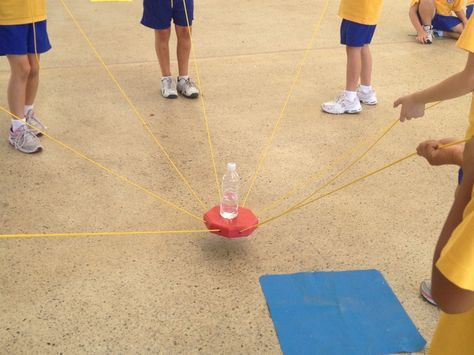
\includegraphics[width=6cm]{4-Solidaire-rouge/sources/81.jpg}
\end{wrapfigure}

But du jeu : Transporter toutes les bouteilles d’un point à un autre

\vspace{0.2cm}

Instructions : chaque joueur tient une ficelle, le maître du jeu pose les bouteilles les unes après les autres sur la plate forme. Si la bouteille tombe il faut revenir au point de départ 
\end{regles}

\begin{imaginaire}

\end{imaginaire}

\begin{moments-stop}
\end{moments-stop}

\end{document}